\documentclass[12pt]{scrartcl}

\usepackage{graphicx}
\usepackage[utf8]{inputenc}
\usepackage{float}
\usepackage{natbib}
\usepackage{euscript}
\usepackage{color}
\usepackage{amsmath}
\usepackage{epsfig}
\usepackage{amssymb}
%\usepackage{graphics}
\usepackage{appendix}
\usepackage[font=footnotesize]{caption}
\usepackage{caption}
\usepackage{subcaption}

\usepackage{hyperref}
\hypersetup{
	colorlinks=true,
	linkcolor=blue,
	filecolor=magenta,      
	urlcolor=blue,
}

%opening
\title{Importance Sampling Tutorial}
\author{Nathan Sanford}

\begin{document}

\maketitle

\begin{abstract}
This short tutorial explains the basics of importance sampling by introducing the concept of Monte Carlo sampling, how importance sampling can be used to apply Monte Carlo sampling to rare events and where these methods are being used in current science. As part of this, I introduce discuss my own research on rare events in a mode-locked laser. This tutorial will hopefully give someone unfamiliar with importance sampling a sense of how powerful it can be, and where to start with applying it to problems.
\end{abstract}

\section{Monte Carlo Integration}

Monte Carlo integration allows one to numerically approximate an integral by drawing a large number of random samples from a probability distribution. For our purposes, consider an integral of the form
%
\begin{equation}
\label{e:expectationIntegral}
I = \int_{D} f(\mathbf{x})p(\mathbf{x})\,d\mathbf{x}
\end{equation}
%
where the integral is over some region $D$ in n-dimensional space and $f$ and $p$ are functions on that space. Additionally, we require that $p$ is a probability density function (PDF), meaning essentially that it is non-negative and integrates to 1 over $D$. Monte Carlo integration works to approximate $I$ by randomly sampling from $p$ and then averaging $f$. For instance, after drawing $N$ samples of $n$-dimensional real random variables from $p$, our approximation to $I$ is
%
\begin{equation}
\label{e:MC_sum}
\hat{I}_N = \frac{1}{N}\sum_{l=1}^N f(\mathbf{X}_l)
\end{equation}
%
where $mathbf{X}_l$ is the $l^{\text{th}}$ sample drawn from $p(\mathbf{x})$. This works as the integral $I$ in Eq. \eqref{e:expectationIntegral} is also an \textit{expected value integral}. 

To make this concrete, let's consider the example of computing the one-dimensional integral
%
\begin{equation}
\label{e:MC_ex}
\mathcal{I}=\int_{0}^\infty e^{-x} \cos(x)\,dx.
\end{equation}
%
If we take $p(x)=\exp(-x)$ to be the probability distribution (note that it is a valid distribution as it is nonnegative and its total integral on 0 to $\infty$ is 1), then the above integral is equivalent to the expectation $\mathcal{I}=E[\cos(X)]$ with $X$ drawn from $p(x)$. Therefore, we can compute the value of $\mathcal{I}$ via Monte Carlo integration by repeatedly drawing samples from the exponential distribution, taking the cosine of each sample, and then taking the mean of all the results. After a sufficiently large amount of samples, we obtain an estimate near the true value of $\mathcal{I}=1/2$. Code for performing this simple example is contained in the folder \texttt{Monte\_Carlo\_in\_C} (written in C). There is code for performing this calculation in serial and \textbf{in parallel} using \href{https://www.open-mpi.org/}{Open MPI}.

Now, the law of large numbers says that $\hat{I}_N$ approaches the true value of $I$ as $N \rightarrow \infty$. However, it will do so rather slowly. The standard deviation of $\hat{I}_N$ is $\mathcal{O}(N^{-1/2})$, meaning that if the number of samples is multiplied by 100, the expected error in the result will only be cut by a factor of 10. That's not a problem for simple examples, but can be especially pernicious in situations where the integration requires many samples to be drawn from the tail of a probability distribution. The relatively low probabilities of such samples exacerbates the scaling of the simulations and makes many applications infeasible. 

As a simple example, let's consider the case of a one-dimensional random walk with normally distributed steps. This problem can be described by a sum of random variables that all are drawn from the Gaussian distribution:
%
\begin{align}
\label{e:1DWalkDef}
Z_J &= \sum_{j=1}^J X_j \quad \text{where the $X_j$ are i.i.d. normally distributed R.V.s} \\ 
\text{so } &p_G(x_j;\mu,\sigma^2) = \frac{1}{\sqrt{2\pi \sigma^2}}\exp{{\Big (}-\frac{(x_j-\mu)^2}{2\sigma^2} {\Big )}} \quad \text{for all } j. \nonumber
\end{align}
%
For simplicity let the mean $\mu$ of every step be 0 and the variance $\sigma^2$ of every step be 1. This dictates that the probability density function of the result after $J$ steps $Z_J$ is also Gaussian-distributed with mean 0 and variance $J$. In other words, the PDF for $Z_J$ is given by $ p_G(z_J;0,J) = (2\pi J)^{-1/2}\exp[-z_J^2/(2J)]$. We can simulate this process with Monte Carlo simulations by drawing samples of the random walk (by drawing $J$ standard normal and summing them) and then binning them to create a histogram which can be compared with the analytical result. Therefore, the integral we are computing using Monte Carlo is 
\[ I=\int f(z_J)p_J(z_J)\,dz\] 
where $p_J(z_J)$ represents drawing samples of the random walk and $f(z_J)$ represents the binning of samples.
The binning process can be thought of as using a series of indicator functions (functions that are 1 over the width of a bin and are 0 elsewhere) in place of $f$. In this way we can re-create the resulting pdf of the random walk after $J$ steps.

The results of Monte Carlo simulations are shown in figure \ref{fig:SimpleGMC} and reflect that the simulation method struggles, relatively, to capture large deviations in the random walk. There are relatively few 
%
\begin{figure}
	\begin{center}
		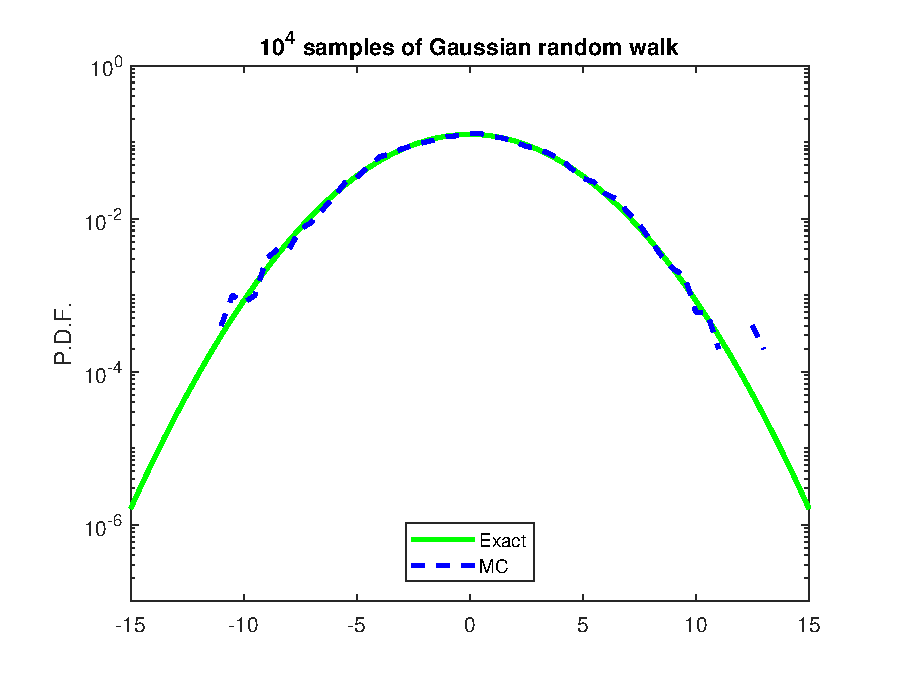
\includegraphics[width=10cm]{GMC.eps}
		\caption[Monte Carlo sampling for the Gaussian random walk.]{Exact and numerical approximations of the PDF of the Gaussian random walk from Eq. \eqref{e:1DWalkDef} with $N=10$ steps and 10,000 samples taken for the numerical approximation. }
		\label{fig:SimpleGMC}
	\end{center}
\end{figure}
%
The 

This can be seen by examining the coefficient of variation (CV) of the simulation. The CV is a measure of the simulation's standard deviation of samples in each bin divided by the probability value in that bin. In this way, it is a probability-adjusted measure of assessing the simulation's variance.

\section{Importance Sampling Basics}

The slow convergence in Monte Carlo simulations for small probabilities can be caused by a mismatch between the function $f$ and the distribution $p$ in Eq. \eqref{e:expectationIntegral}. Obviously, the integral $I$ will be dominated by regions where $f$ is approximately maximal, and in many cases $p$ is not maximal in the same region. When this happens, the ``important" regions for $f$ are undersampled and the estimate $\hat{I}$ converges very slowly. An augmentation to MC simulation called importance sampling (IS) corrects for this by introducing an artificial probability distribution, called a biasing distribution, into the simulation from which samples are drawn \cite{Bucklew2004}. The goal of this technique is to replace $p$ with a distribution that heavily weights regions of probability space where events of interest occur most often.

The insight which makes IS possible is that Eq. \eqref{e:expectationIntegral} can be rewritten as
%
\begin{equation}
\label{e:biasedIntegral}
I = \int_{\mathbb{R}^n} f(\mathbf{x})\frac{p(\mathbf{x})}{p^*(\mathbf{x})}p^*(\mathbf{x})\,d\mathbf{x}.
\end{equation}
%
The function $p^*$ is the biasing distribution and will be treated as given for this discussion. The choice of biasing distribution is an application specific problem and investigating rationales for choosing biasing distributions is a rich field of inquiry in many contexts. Once a biasing distribution is chosen we perform MC simulations by drawing samples from $p^*$ and then computing
%
\begin{equation}
\label{e:ISMC_sum}
\hat{I}_N = \frac{1}{N}\sum_{l=1}^N f(\mathbf{X}_l)\frac{p(\mathbf{X}_l)}{p^*(\mathbf{X}_l)}.
\end{equation}
%
In an ISMC simulation, the sample results are now weighted by the likelihood ratio, or 
%
\begin{equation}
\label{e:likeRat}
L(\mathbf{X}_l)=\frac{p(\mathbf{X}_l)}{p^*(\mathbf{X}_l)},
\end{equation}
% 
which corrects for the fact that samples were drawn by the biasing distribution and gives results equivalent to if the original distribution had been used. 

The success of importance sampling is principally judged by two factors: that the resulting integral or probability computed is reasonable, and that the convergence is suitably fast. The second criterion can be addressed by examining the variance of the IS integrand
%



\section{Research for Large Deviations in Complicated Systems}

\end{document}
